%%%%%%%%%%%%%%%%%%%%%%%%%%%%%%%%%%%%%%%%%%%%%%%%%%%%%%%%%%%%%%%%%%% 
%                       rpithes-short.tex                         %
%         Template for a short thesis all in one file             %
%        (titlepage info below assumes masters degree}            %
%  Just run latex (or pdflatex) on this file to see how it looks  %
%      Be sure to run twice to get correct TOC and citations      %
%%%%%%%%%%%%%%%%%%%%%%%%%%%%%%%%%%%%%%%%%%%%%%%%%%%%%%%%%%%%%%%%%%% 
%
%  To produce the abstract title page followed by the abstract,
%  see the template file, "abstitle-mas.tex"
%
%%%%%%%%%%%%%%%%%%%%%%%%%%%%%%%%%%%%%%%%%%%%%%%%%%%%%%%%%%%%%%%%%%%

\documentclass{thesis}

\usepackage{graphicx}   % if you want to include graphics files
\usepackage{cite}

% Use the first command below if you want captions over 1 line indented.
% A side effect of this is to remove the use of bold for captions. 
% To restore bold, also include the second line below.
%\usepackage[hang]{caption}     % to indent subsequent lines of captions
%\renewcommand{\captionfont}{\bfseries} % only needed with caption package;
                                        %   otherwise bold is default)

%%%%%%%%%%%%%%%%%%%%  supply titlepage info  %%%%%%%%%%%%%%%%%%%%%

\thesistitle{\bf Acoustics Visualization\\For Architectural Spaces}        

\author{Max Espinoza}        

\degree{Phd in Computer Science} 

\department{Computer Science} % provide your area of study here; e.g.,

%  "Mechanical Engineering", "Nuclear Engineering", "Physics", etc.

\thadviser{Dr. Barbra Cutler}
% \projadviser{Dr. Barbra Cutler}

%\cothadviser{First co-adviser} %if needed

%\cocothadviser{Second co-adviser} % if needed

%  For a masters project use \projadviser instead of \thadviser, 

%  and \coprojadviser and \cocoprojadviser if needed. 

\submitdate{May InsertYear\\(For Graduation InsertDate)}        

%\copyrightyear{1685}  % if date omitted, current year is used. 

%%%%%%%%%%%%%%%%%%%%%   end titlepage info  %%%%%%%%%%%%%%%%%%%%%%

      

\begin{document} 

\titlepage             % Print titlepage   

%\copyrightpage        % optional         

\tableofcontents       % required 

% \listoftables          % required if there are tables
% \listoffigures         % required if there are figures


%% ╔╦╗╔═╗╔╦╗╔═╗
%%  ║ ║ ║ ║║║ ║
%%  ╩ ╚═╝═╩╝╚═╝

%%%%%%%%%%%%%%%%%%%%%%%%%%%%%%%%%%%%%%%%%%%%%%%%%%%%%%%%%%%%%%%%%%%%%%%%%%%%%%%
% Acknowledgment                                                            
%
%\specialhead{ACKNOWLEDGMENT}
%this heading is not numbered.

%%%%%%%%%%%%%%%%%%%%%%%%%%%%%%%%%%%%%%%%%%%%%%%%%%%%%%%%%%%%%%%%%%%%%%%%%%%%%%%
%% Abstract                                                                  
%%%%%%%%%%%%%%%%%%%%%%%%%%%%%%%%%%%%%%%%%%%%%%%%%%%%%%%%%%%%%%%%%%%%%%%%%%%%%%%
\specialhead{ABSTRACT}

% One Sentence Topic (Try number 1)
Interactive visualization of sound propagation in architectural spaces offers architects an iterative approach to construct room designs with desired acoustical proprieties through changes in geometry and materials in simulated models.

% Research question
We are investigating methods to simulate and visualize sound propagations with interactive frame rates for varying geometries with uniform sampling densities throughout simulation.

% What we are doing that is new / different
Simulating sound wave propagations can be done in real time with existing algorithms, however these algorithms require intensive offline computation for each new room geometry simulated.
% TODO: Fix "noisy" visualization doesn't sound right
There exist geometrically based algorithms that do not require off line computation, however yield noisy visualizations, require a large initial sampling, or do not capture all acoustical phenomenons; 

% How did we tackle this question Extending wave
Wave particles\cite{Yuksel2010}, introduced by Cem Yuksel for real-time  water simulation through rendering extended height fields, can be used to simulate the wave front propagations of sound offering visualizations at interactive frame rates for use in an iterative designs of room geometries.

% How did we go about this 
We created a design tool for architecture students that will allow the  creation of 3D models and interactive visualizations of sound wavefronts in created spaces given an source position.

% Impact of research 
With this toolkit designers will be able to assess the general acoustical properties of a room in the early design phase. Furthermore with support of BDRFs found in commercial wall materials that will allow designers to creatively use these to achieve desired acoustical properties.

%%%%%%%%%%%%%%%%%%%%%%%%%%%%%%%%%%%%%%%%%%%%%%%%%%%%%%%%%%%%%%%%%%%%%%%%%%%%%% %% Introduction                                                             
%%%%%%%%%%%%%%%%%%%%%%%%%%%%%%%%%%%%%%%%%%%%%%%%%%%%%%%%%%%%%%%%%%%%%%%%%%%%%%
\chapter{Introduction}

Architectural acoustics is a branch of engineering that relates to the science behind the generation of specific sound properties in architectural spaces. Architects and professional acoustical consultants are involved with architectural processes in two practices . \\

First, Professional consultants evaluate the acoustics of an architectural space in order to modify sound properties within the space. This is done through use of sound absorbers, changes of floor and ceiling materials, or other sound altering techniques.\\

Secondly, Architects take into consideration the acoustical properties within the early stages of the design and have far greater control over the geometry and location of rooms than those consultants fixing unwanted sound properties in space post construction. Architects meeting client needs preemptively know the location and functions of rooms and can move those locations in order to achieve noise isolation. Furthermore if architects are planning for sound to travel further into a room they can plan for reverberations through room geometries and materials. The advantages in being able to plan and estimate the acoustical properties of a given space before construction are two fold. Unwanted acoustical properties can be detrimental to building residents and businesses.\\

Echoes in the workspace or loud street noises in a residential apartment can causes a reduction in the utility of the space. Secondly, many of these mistakes must be later fixed through use of acoustical absorber, special drywall materials, and insulation. All of which cost the client capital. Hope Bagenal Author of the Practical Acoustics \cite{Begenal} published in 1940s writes that “structural sound insulation has been little understood but remains technically difficult and expensive.” He goes on to state that “it is cheaper to conquer noise by segregation and separation.” While sound insulation is much better understood since Bagenal wrote in his handbook a generation ago that it is still cheaper to plan for given acoustical properties of a space then fix issues post construction.\\

The planning for acoustical properties in a given space is no easy task. Acoustics are hard visualize and understand especially for complex spaces due to sound wave behaviors such as reverberation, diffraction, refraction and absorption. While architects are trained in the basic of sound behavior, the use computer software to run acoustical simulations on their virtually created spaces results in more accurate predictions of acoustical properties. \\

Simulation software such as Grasshopper\cite{grass}, a plugin for Rhino 3D modeling tools,  offer designers the ability to run acoustic simulations on virtually designed spaces. Given that the architectural design process is iterative, simulations must be provided relatively quickly to promote creativity and allow designers to explore the effects of changing their design on the acoustical properties of their virtual space. Rendering the results of these simulations as visualizations or auralization are provide useful feedback to designers. The ability to visualize sound propagation through a given space gives designers insight into improving designs for noise isolations, fixing unwanted reverberations, and planning acoustical reflections.\\

Architecture 3D modeling software tools such as Rhino, AutoCad Architecture, and AutoDesk Revit Architecture are mature software that contain many features for building models. However due to the complexity of building models using sophisticated software, users tend to take longer periods of time creating simpler models  the is needed for the initial exploration of room geometries and layouts. Previous research done for lighting visualizations allows user to use physical primitives to sketch a room model on a tabletop interface. \cite{josh} With the extension of a user interface, designers can create closed models through drag and drop 2D representations of those primitives to sketch a 3D geometry of a given room within a few seconds.  Furthermore the tools required to build models that most acoustical simulations use as input are time intensive, taking away designers ability to creatively explore renovations on their model at interactive rates.\\

There exist several algorithms for the simulation of acoustic  in architectural spaces, however many of these algorithms geared at interactivity do not simulate some acoustics behavior, such as diffraction.
Using models created through placement of primitives in a web interface we explore how to improve existing algorithms such as phonon tracing \cite{bertram} to handle sound behaviors such as diffraction.\\

We believe that if we can simulate a wavefront through the use of wave particles  in a phonon mapping based simulation then we can offer a wider range of visualization while capturing properties that most real-time algorithms for acoustics simulation do not.
%join
Since we are focused on the visualization portion of this research for our class final project and wave particles have yet to be fully implemented at the time of writing this report I will focus more on what was discussed during the final presentation.\\

%%%%%%%%%%%%%%%%%%%%%%%%%%%%%%%%%%%%%%%%%%%%%%%%%%%%%%%%%%%%%%%%%%%%%%%%%%%%%% %% Related Works
%%%%%%%%%%%%%%%%%%%%%%%%%%%%%%%%%%%%%%%%%%%%%%%%%%%%%%%%%%%%%%%%%%%%%%%%%%%%%%

\chapter{Related Works}
There were many papers I took into consideration when researching the topic of acoustical simulation. There were two main approaches to solving the problem of simulating wave propagation in a 3D space.  On method was numerically solving the wave equation, which yields the most accurate results because the wave equation captures all wave behaviors including diffraction and interference. However this usually required voxelation of the scene and an expensive offline computation that could range in a few minutes to hours. Even research boasting interactive framerates for acoustic simulations had an offline component for each new geometry the simulation was run on. Considering we wanted to encourage designers to change the geometry of a room with no additional computational cost we needed a faster approximation approach. 
Geometric acoustical simulations make the assumption that sound acts like a ray and components such as diffraction are later taken into consideration. This allows us to use rays instead of having to solve the computation expensive wave equation. However, this is a visualization class, so we will also focus on the different visualizations used to show designers something about the acoustical properties of their design.

\section{Image Method}

The Image method developed in 1978 was one of the first acoustics simulations algorithms developed for computer aided design\cite{Allen1979}. It was fast and efficient, however was limited to box shaped rooms. Later this was extended to handle arbitrary polygonal shaped rooms, with performance losses. The idea behind this algorithm is that a sound ray when leaving a source and hitting a surface has the same properties as sound ray that originated in the mirrored direction with loss of energy due to absorption taken into account. These image sources are constructed for multiple reflection and later used to determine whether these mirror image sources can be heard a receiver in the scene. After a visibility test you consider all the virtual image sources that affect that listener to obtain acoustical benchmarks. As stated before while this is efficient on box shaped rooms, it suffers greatly when dealing with a room that is represented as triangulated mesh with complex geometry. As a result this method isn’t used in favor of more flexible and efficient methods for the models created by architects. 


\section{Beam Tracing}

Beam tracing\cite{Funkhouser2004} was introduced by Thomas Funkhouser in 2004 as an extension of ray tracing used for architectural acoustics simulations.  A large issues in ray tracing in both sound and lighting simulations it requires a large number of rays to be shot into the scene from a source. The more rays you shoot into the source the less noise you have to deal with in the final rendering/simulation results. Therefore using ray tracing techniques usually meant the you couldn’t have an interactive rates because a dense sampling of the space was required to obtain accurate results. However instead of tracing a ray, you could trace a convex polyhedral beams from the location of sound sources. These beam traces wouldn’t suffer of undersampling problems rays have, as a single beam can be used in place of infinitely many rays. It scales to support large environments and can even model wedge diffraction.


\section{Morphable Sphere}

Design and Outcomes of an Acoustic Data Visualization\cite{Rob} is a paper that covers an Applied Data Analysis and Visualization seminar offered in Aalto University of Science in Aalto Finland catered to students with some background in computer graphics.  These students were given  spacial room impulse response of Europe ten great concert halls gathered in the year 2012. The data was collected through the use of multiple loudspeakers and omni-directional receivers. Using of the Spatial Decomposition Method they were able to capture high dimensional data such as the monaural pressure impulse response, and 3 dimensional directional components of the sound arrival direction vector for each sample in one monaural impulse response.

Monaural pressure impulse response refers to the changes in pressure as a response to an impulse, sound being generated, in an architectural space. This response describes the reaction of the system as a function of time.

“Students were encouraged to explore visualizing source positions, receiver positions, spatial aspects, with temporal development of the sound field, frequency characteristics, and comparison between halls.” 

The sound field is a space in a medium, usually air in architectural acoustics, where sound waves are being propagated.

There were three projects in this seminar, of which make creative use of color and shapes to represent higher dimensional sound data. Peteri Leskinen made a nested tessellated spheres visualization of broadband sound data.  Broadband sound data is sound in many frequencies, as opposed to octave where you segment lower frequencies form the higher ones. The white noise generation we use as one of our sources is also considered a kind of broadband sound.
Leskinen took a uniform sphere and with precomputed data and manipulated the vertex positions in relation to energy in each direction over a specific time window. Earlier times could be nested inside later time windows and through use of transparency allow users visualize the change in the direction of sound temporally in a static image.

Leskinen visualization has the same goal as this our visualization, however his morphable sphere only gives a general direction of where sound comes from. Phonon mapping gives users more insight into how the geometry of a room effects sounds propagations, including early reflections and late reverberations.  Furthermore Leskinen visualization isn’t a simulation, it requires captured data, that needs to be processes to work through is web interface.  On the other hand we take in geometry as input and simulate sounds interaction to generate similar visuals without the need of complex arrays of speakers and microphones and already built spaces. 

\section{Phonon Tracing}

Another visualization technique, partially implemented in my visualization, is phonon tracing \cite{bertram} introduced by Martin Bertram in 2005. Given a geometry, source, and listener position this simulation method returns a finite impulse response filter. This response filter is the result of sounds complex interaction with the geometry of the room and various surfaces with frequency-dependent absorption coefficients. Furthermore Bertram can use these filters to create an auralizations of sound in the environment. For this project I concern myself with the visualization portion of Bertram’s algorithm. 

Phonon tracing is accurate for mid- and high-frequency sound, however low frequency sounds are not handled in phonon tracing.  The visualization behind the simulation uses colored blobs to trace the path created by a phonon throughout the space as it bounces of the room’s geometry. Many of these blobs allow users to see the wavefront propagation temporally.  Bertram uses color to visualize the spectral energy of phonons; phonons with low frequency are depicted as blue, medium frequency as green, and high frequency as red blobs.  Furthermore the darker the color of a phonon gets represents how much energy has been absorbed by the materials it has been interacted with.

Changes in frequency happen when phonon interact with materials in the scene that change the reflected phonon spectral energy. Bertram shares our same objective, in that given virtual models we want users through analysis to improve the sound properties the space through changing model's geometry or materials. Users can interact with this simulation by using a slider to go through time and visualizing the phonons corresponding to a Dirac, a unit impulse,  sent out from the initial source.  

The biggest limitation of Bertram’s method is that it cannot capture phenomena that occur with lower frequency sound such as diffractions. A phenomenon we attempt to capture in our visualization through splitting of phonons as wave particles. The author claims that for the analysis of acoustic clarity of sound,  lowest frequencies can often be neglected, however this is not always the case for noise isolations.

In phonon tracing each photon carries the following information with it:  a spectrum of energy, distance traveled from source, its current position, and outgoing direction. My visualization being an extension of phonon tracing also have phonon that contain the same information throughout the simulation.  However, we take into account splits and merges that occur because of our desire of having more phonon to later create a surface mesh over for visualization purposes, and to better capture sound behaviors like diffraction. Due to this we could not not take shortcuts introduced in this paper to increase the performance of phonon mapping.  We use phonon mapping as a base to to implement wave particles and capture more acoustical phenomenon.


\section {Wave Particles} 

Our paper is also an extension of Wave Particles into 3D used for acoustics simulations \cite{Yuksel2010}.  Wave particles are originally used to create an extended height field of interactive real-time fluid simulations.  Wave particles are implemented to be fast, easy to code, and unconditionally stable way to approximate a wave simulation. Furthermore Yuksel accounts for local wave induced flow by warping this extended hight field. With the use of modern graphics hardware to accelerate the process of generating this height field, real time frame rates can be achieved for hundreds of buoyant objects in the water simulation.  The cornerstone of this paper is using wave particles to model complex wave interactions by computing the local deviation functions required to solve the wave equation. 

Usually simulations solving wave equations require more computationally expensive algorithms, however Cem reduces this to a keeping track of wave particles propagating throughout a 2D plane. These wave particles each carry a radii, amplitude, position, and direction. Note that these attributes are similar to those carried in phonon tracing.  Cem Yuksel use of wave particles give us the idea of splitting phonon so that we can overcome the under-sampling problem phonon mapping experiences. In addition later we with this uniform phonon map we can wrap a mesh around phonons in order to visualize the wave front as a smooth surface interacting with the given geometry. 

However, Yuksel formulates wave particles to be as independent as possible, in order to achieve greater efficiency to render in real time. As a result diffraction is not taken into consideration and ignored. Instead conditions where diffraction might affect the outcome of the simulation are avoided.

To handle phenomenon such as diffraction, one must into account each particles neighbors that requires much more computationally expensive tracking. Reducing the overall efficiency of the algorithm, and making it less parallel and portable to GPU. Considering we are trying to handle diffraction in 3D, this is a major drawback to using wave particles. 


%%%%%%%%%%%%%%%%%%%%%%%%%%%%%%%%%%%%%%%%%%%%%%%%%%%%%%%%%%%%%%%%%%%%%%%%%%%%%% %% Algorithms
%%%%%%%%%%%%%%%%%%%%%%%%%%%%%%%%%%%%%%%%%%%%%%%%%%%%%%%%%%%%%%%%%%%%%%%%%%%%%%
\chapter{Implementation}
As mentioned previous we wanted to extend wave particles through the use of phonon mapping in a geometry representative of an architectural space. Given that we wanted to incorporate previous research we used models generated by our web based user interface for daylighting simulations. 

Firstly, this project required the ability to load a mesh in OBJ standard format and parse it such that we can differentiate between structures in a room, such as the ceiling, individual walls, windows, floor, and extra geometries. OpenGL was used  because of existing frameworks and data structures that aided in loading meshes and more importantly OpenGL can handle much larger element on the screen then other graphical tools such as Processing and OpenFrameworks. 

Secondly, we needed to implement particles moving within the scene and collision detection in order to implement phonon mapping. 
We used the ray tracer data structure provided in previous assignments to aid in this implementation. In addition we needed to incorporate absorptive materials and account for the resulting changing sound intensity after collisions with materials. 

Lastly, we needed to implement wave particles and how they would fit into phonon mapping. We related individual phonon to the wave particles used in water simulation and showed how despite significant reduction in performance they later can be optimized to account for sound behaviors such as diffraction. The mesh that wave particles provide can later leverage for other visualization techniques. Such as fitting a surface to points that make up a wave front for clearer visuals then sparse point data. Most of this is outside the scope of this visualization class, and will be talked about briefly later in this report.

\section{Meshes}

Loading the mesh into the scene was not difficult as I already had code that could load triangle meshes, saved as OBJ files, into OpenGL. A side note I used GLFW and GLM for all my display controls and math libraries, both modern tools for programing in modern OpenGL. One difficulty I had was finding a way to differentiate between walls in the scene. Since all the walls in the OBJ files were categorized as a single wall. Updating an intermediately file to explicitly label each wall with a different material in the OBJ worked. From that we could parse what wall each triangle in the scene belonged too. We created a wire frame visualization to confirm that our mesh is loaded in correctly.
 \begin{figure}
        \centering
        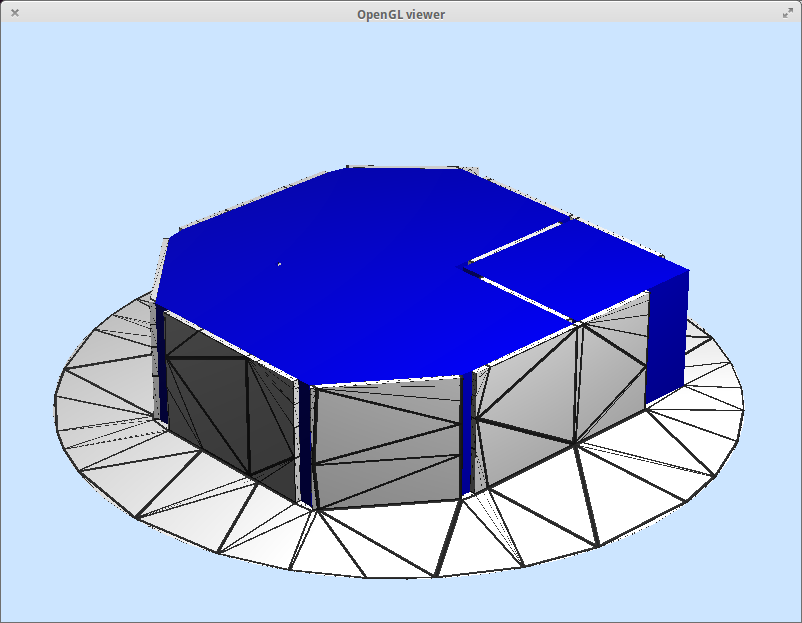
\includegraphics[width=2.5in]{images/wireframe}
        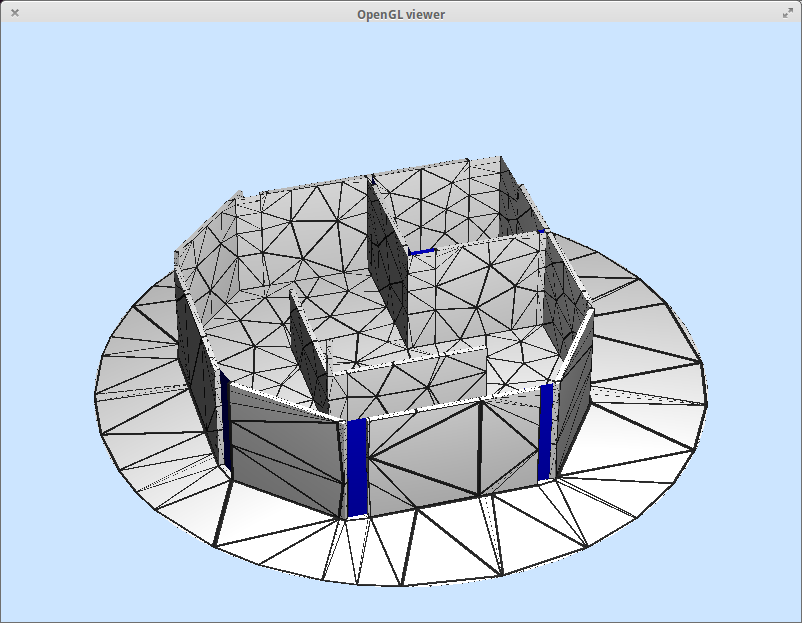
\includegraphics[width=2.5in]{images/wireframe_open}
        \caption{The wire frame rendering of the meshes of an example mesh loaded into OpenGL. Toggling off between viewing the ceiling and inside the space}
    \end{figure}
%lms picture

\section{Phonon Mapping}
The phonon in Bertram paper carry the same attributes as ours such as: direction, position, intensity, and frequency. For the intensity I choose to use wattage in order to represent an amount of work each phonon is doing on the air around. Bertram, in aiming to create an audio  based aurilization creates his own unit of measurement for phonon, however we are currently only interested in visualizing sound waves. Phonon being a representation of work on a medium such as air, are shot into the scene.  Their wattage remains constant until a collisions with a material. Then that material  adsorbs a specific percentage of a phonon intensity depending on the phonon's frequency. Only the frequency remains static over the simulations. And frequency is represented in Hz, from 20Hz to 20kHz.

To save time in computation whenever a phonon is created we calculated how many time steps it would take a phonon to reach the closest wall in its path. The phonon then moves each time step until its internal timer reaches zero and program knows the phonon hit it's closet wall. We then computed the reflection angle and set the phonon for the next collision. Because of this we only get drop in frame rates when a lot of particles hit walls at the time. 

Even more we are trying to make a scientific tool, therefore placement of the particle was computed from where the particle collided with the wall and  and then moved the particle depending on how much time time was left after the phonon collision within that single time step. This is to ensure the most accuracy we get while using doubles to store positions and times.  

Also, the phonon mapping paper includes piecewise functions of material absorption coefficients that we used to compute how the intensity of each particle change as a function of frequency.
% picture of charts
\begin{figure}
        \centering
        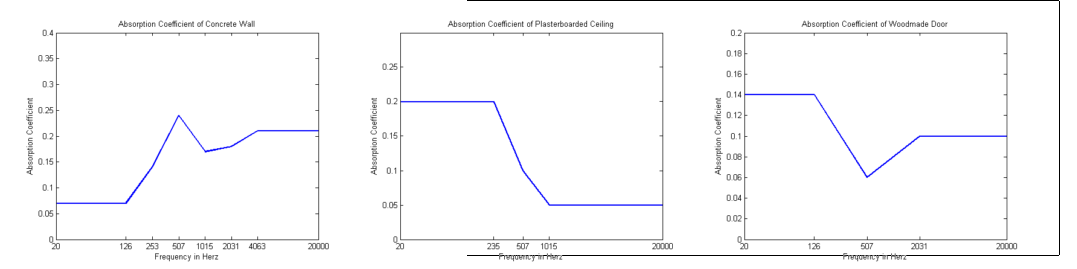
\includegraphics[width=5in]{images/chart_1}
        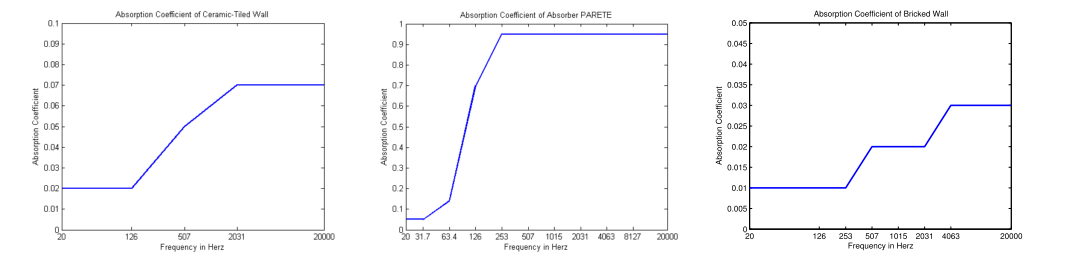
\includegraphics[width=5in]{images/chart_2}
        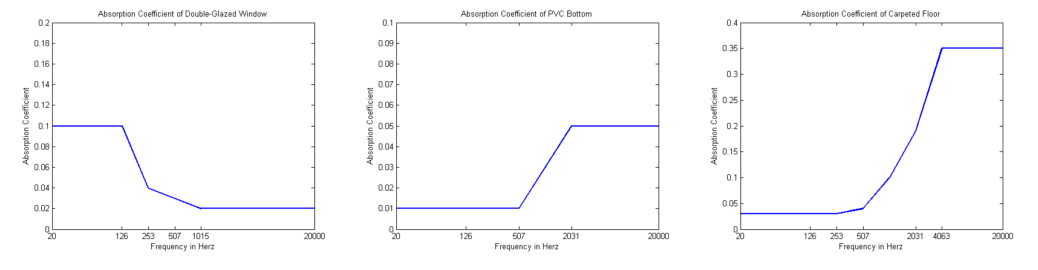
\includegraphics[width=5in]{images/chart_3}
        \caption{The absorption functions for the materials we implemented in our simulation. This graph was featured in Bertram phonon tracing paper.\cite{bertram}}
    \end{figure}
    
Time was also spent exploring different visualization methods, of which proved to be difficult as the range of sound from 20Hz to 20kHz is very large. I then convert intensity of each particle into a logarithmic scale to give more informative visualizations. Seeing I used wattage to represent the intensity of a phonon I converted wattage to decibels, which relates closely to how we hear in a range from 0db to 120dBs.
\begin{figure}
        \centering
        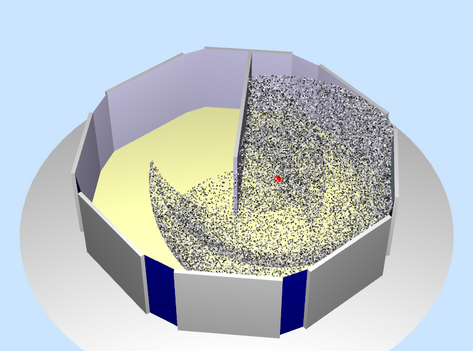
\includegraphics[width=2.845in]{images/freq_show}
        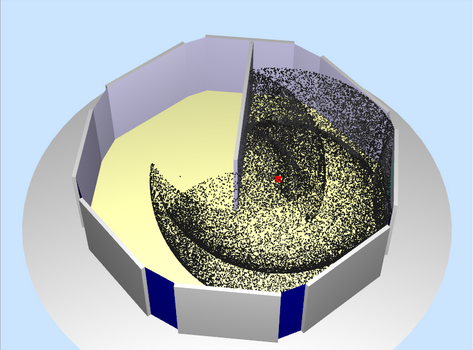
\includegraphics[width=2.845in]{images/intensity_show}
           \caption{On the left is the frequency visualization of white noise, on the right
           is the intensity visualization set at 120dBs}
    \end{figure}
    
I worked on three kinds of visualizations from simulation results. In the frequency visualization I mapped black to high frequencies noises at 20kHz and low frequency noises to white at 20Hz. This is useful for seeing the differences in frequencies distribution between sound sources. As can be seen in Fig 3.3. Secondly I did a similar mapping for intensity, I mapped black as being the most intense at 120bBs and white as being least intense as 0dbs. I then created a hybrid where I mapped low frequency phonon with to the color blue, and medium frequency to the color green, and higher frequency to the color red. I also wanted to show the intensity of a phonon, which I mapped into the alpha value. 
%Random picture of hybrid system
\begin{figure}
        \centering
        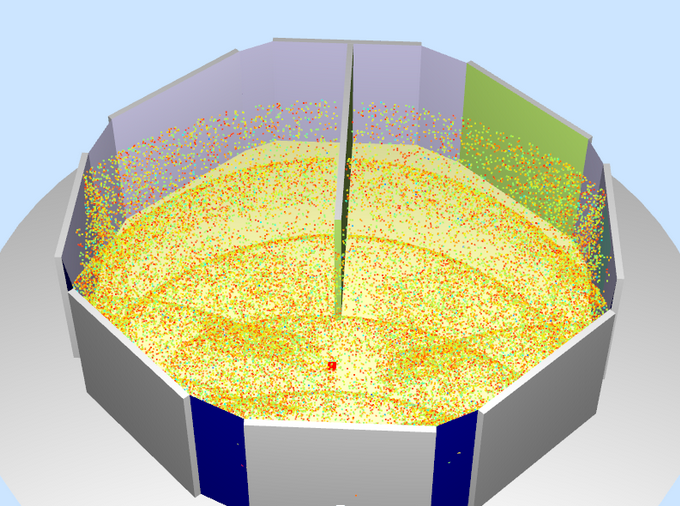
\includegraphics[width=2.845in]{images/hybridVis_show}
        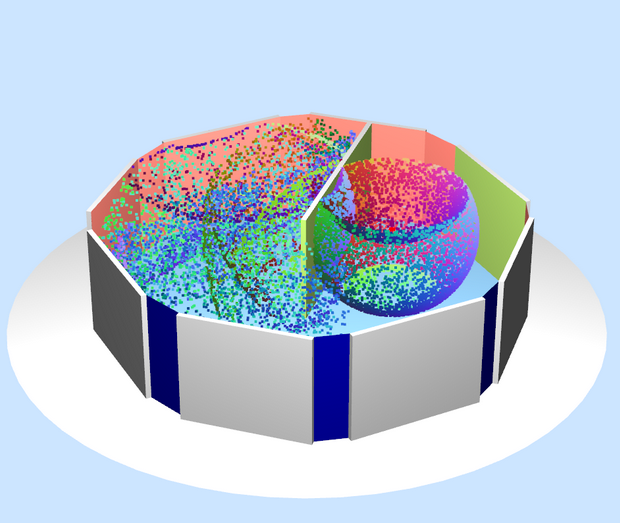
\includegraphics[width=2.5in]{images/wave_show}
        \caption{On the left is the hybrid visualization mode that uses colors to show particles frequencies and alpha values to show intensity. On the right there is the wave front visualization of two expanding waves.}
    \end{figure}
    \begin{figure}
        \centering
        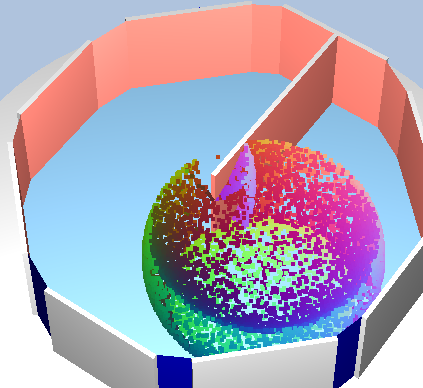
\includegraphics[width=1.5in]{images/wave_1}
        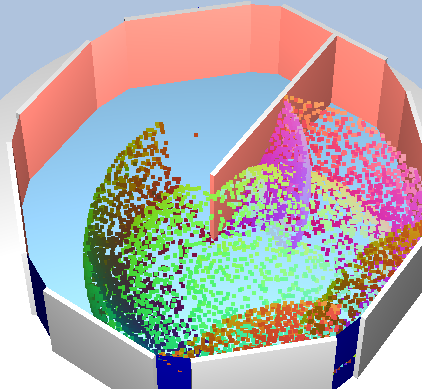
\includegraphics[width=1.5in]{images/wave_2}
                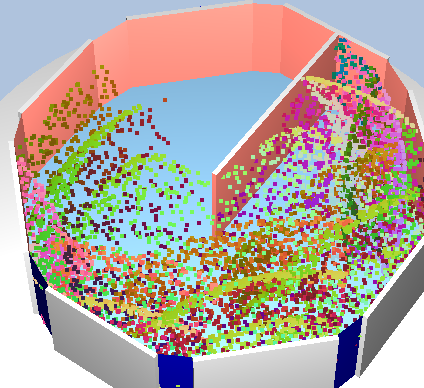
\includegraphics[width=1.5in]{images/wave_3}
        \caption{Wave visualization, you can see t
        hat once a wave front hits a wall those other particles that hit also share similar colors.}
    \end{figure}
    
    
Lastly for the direction visualization I mapped RGB color space to the X Y and Z component of each particle's direction. This yielded in a smooth transition between directions and makes viewing static images of the phonon map much clearer because you can distinguish between different 3D waves fronts  in the simulation. 

\section{Wave Particles}
Wave particles proved to be difficult and more work it needed to fully implement them into our simulation. The wave particles created recursive patterns that despite being pretty are not useful in representing a wave as a collection of points on a sphere.


%%%%%%%%%%%%%%%%%%%%%%%%%%%%%%%%%%%%%%%%%%%%%%%%%%%%%%%%%%%%%%%%%%%%%%%%%%%%%% %% Results
%%%%%%%%%%%%%%%%%%%%%%%%%%%%%%%%%%%%%%%%%%%%%%%%%%%%%%%%%%%%%%%%%%%%%%%%%%%%%%
\chapter{Results for Final Project}

Overall for this visualization project I achieved my goal of setting up the framework for my graduate research. I’ve implemented phonon tracing with realistic material properties on objects in the scene, however I did not finish the implementation of transforming the phonon into wave particles. The splitting of the each wave particle and rules that direct those splits require more work and debugging to figure fully implement. In addition need still implement merging of particles, to prevent the wavefront bring becoming higher resolution in specific locations. We were able to gather some interesting results though, running our simulation for 
10,000
iterations we were able to see some expected results in the visualization due to the differences in wall materials and sound source. Below we show some examples and a brief explanation as to why results match our expected institution of the scene. 

\section{Carpet floor vs PVC floor}
Given that carpet has many filaments that not only cause diffuse reflection with light, but also diffuse reflections of sound. Carpet absorbs more sound than plastic flooring so we should see that the intensity of the phonon are reduced much faster than in the carpet simulation. Which is clear from the second column on figure 4.4.

%Picture of Carpet floor in Freq mode, Intensity Mode, Hybrid Mode
%Picture of PCV floor in Freq mode, Intensity Mode, Hybrid Mode
\begin{figure}[H]
        \centering
        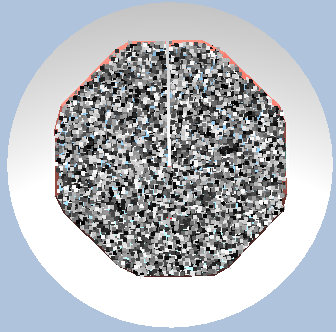
\includegraphics[width=1.55in]{images/freq_carpet}
        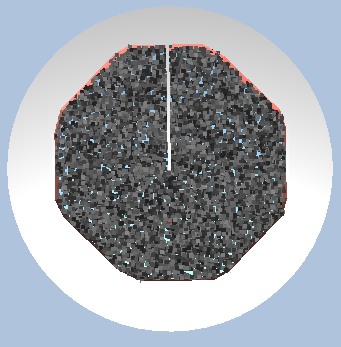
\includegraphics[width=1.5in]{images/intensity_carpet}
        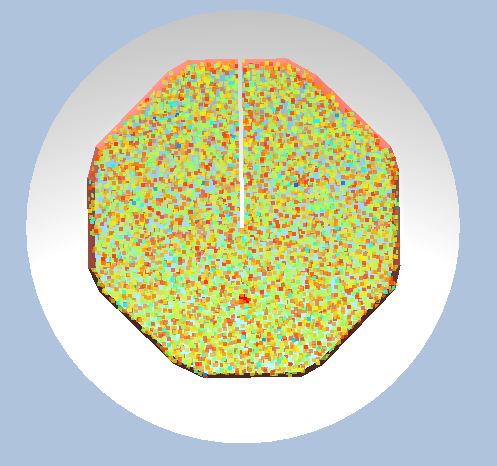
\includegraphics[width=1.63in]{images/hybridVis_carpet}
        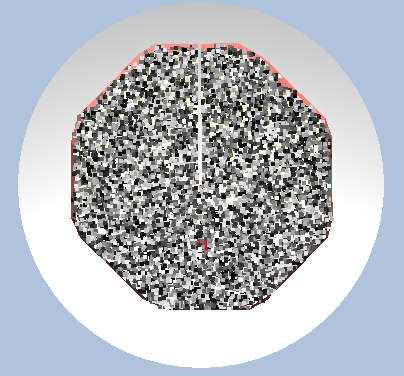
\includegraphics[width=1.6in]{images/freq_pvc}
        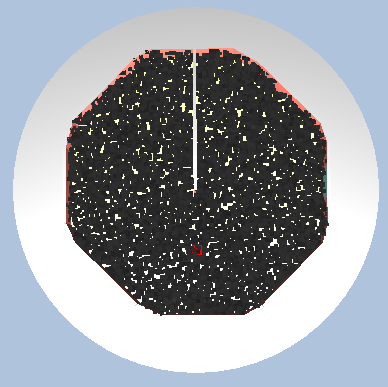
\includegraphics[width=1.5in]{images/intensity_pvc}
        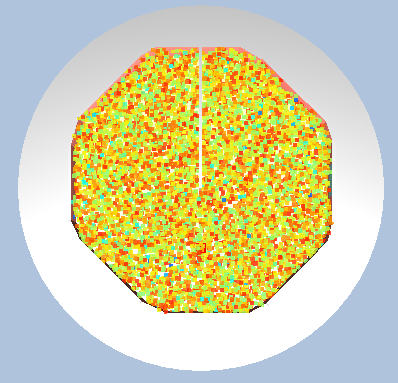
\includegraphics[width=1.55in]{images/hybridVis_pvc}
        \caption{On the top are the results for carpeted floor and on the bottom for plastic based floors.}
    \end{figure}
    
    \begin{figure}
        \centering
        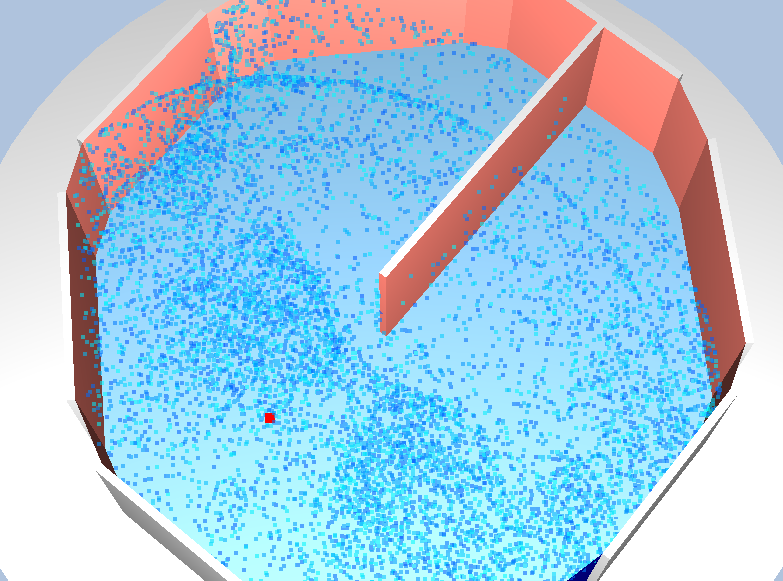
\includegraphics[width=1.5in]{images/low}
        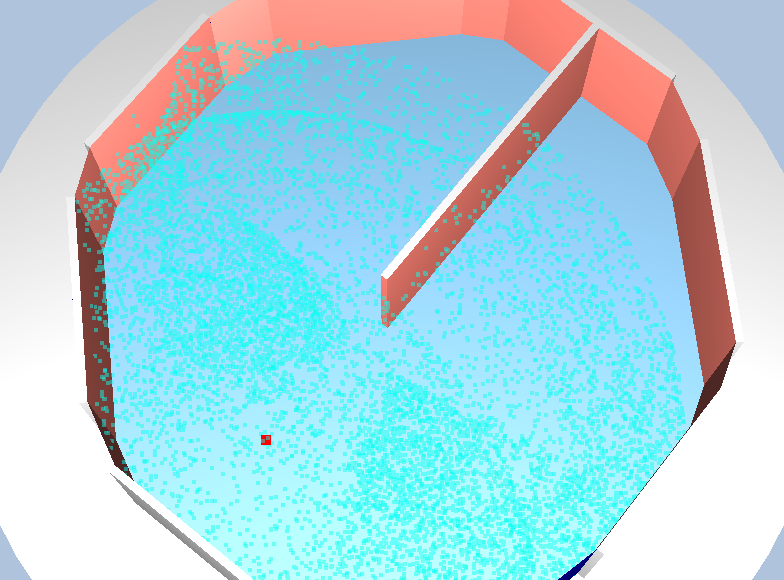
\includegraphics[width=1.5in]{images/med}
        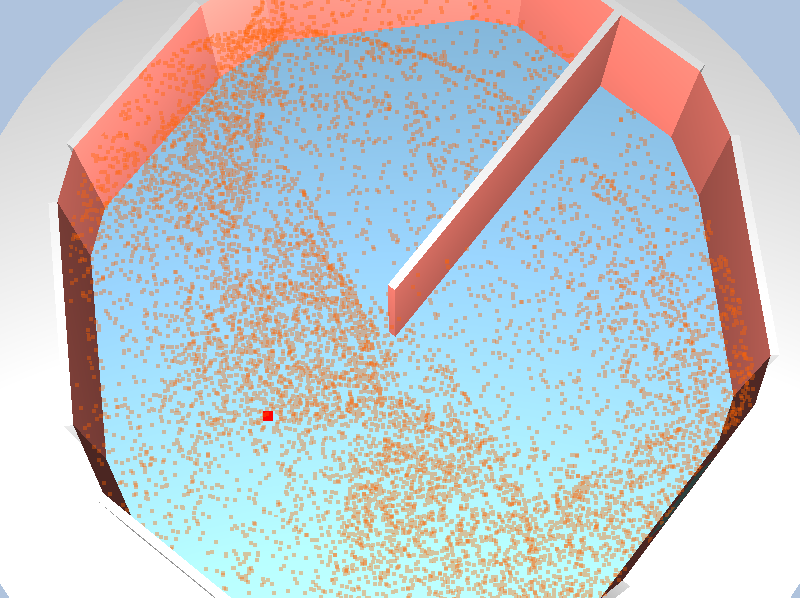
\includegraphics[width=1.5in]{images/high}
        \caption{We also had implemented different kinds of sound source varying in decibels from low hums to loud talking. In addition we also matched the foundation frequency of these sound sources. Here are those presets viewed from left to right:AC humming at 70dBs with a low frequency, People talking at 60dBs mid range frequencies, and the high pitch of CTR monitor at 40dBs}
    \end{figure}

\section{ Concrete vs Ceramic Tile}
Just as above, according the absorption function ceramic tile is a horrible absorber of sound. Out of all the material tests ceramics are absorb the least amount of noise. On the other hand surprisingly concrete usually absorbs about a fourth of all sound in most frequencies. So we should expect to see that in intensity of the particles in the concrete figures reflect this.
I was surprised to see the results that what looks like similar results in from using both materials. 

%Picture of Concrete in Freq mode, Intensity Mode, Hybrid Mode
%Picture of Ceramic floor in Freq mode, Intensity Mode, Hybrid Mode

\begin{figure}
        \centering
        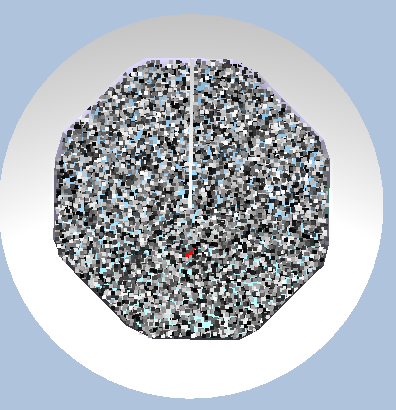
\includegraphics[width=1.4in]{images/freq_cem}
        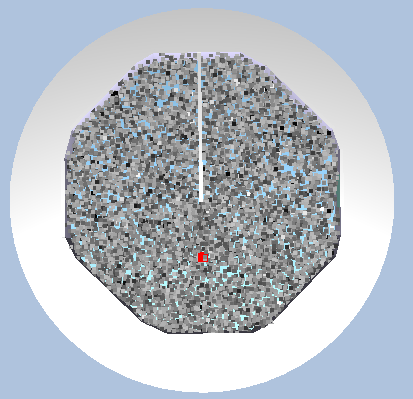
\includegraphics[width=1.5in]{images/intensity_cem}
        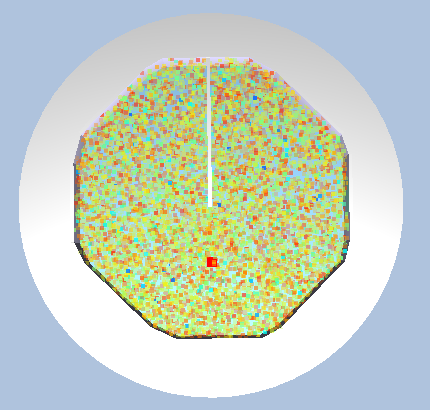
\includegraphics[width=1.5in]{images/hybridVis_cem}
        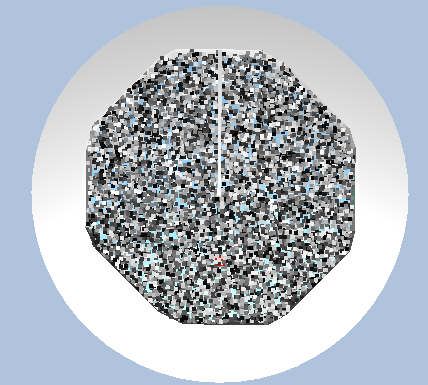
\includegraphics[width=1.5in]{images/freq_tile}
        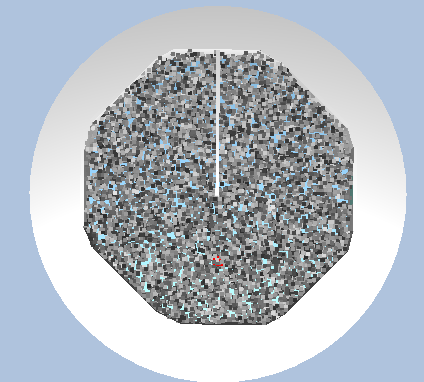
\includegraphics[width=1.5in]{images/intensity_tile}
        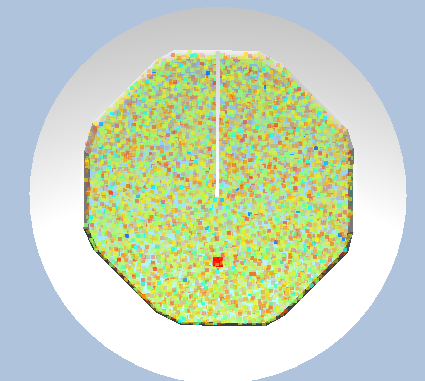
\includegraphics[width=1.5in]{images/hybridVis_tile}
        \caption{On the top are the results of a room with cement walls, and on the bottom with tiled walls installed.}
    \end{figure}
\section{Concrete room with absorbers \& without absorber }
The absorbers are an amazing material that absorbs about 90\% of all sound in wavelengths above 126Hz. We should see that in the room with these absorbers that sound dissipates rather quickly. 
\begin{figure}
        \centering
        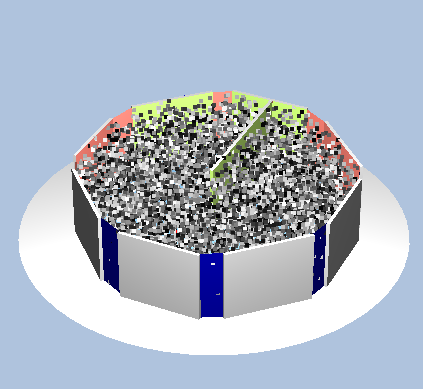
\includegraphics[width=1.5in]{images/freq_abs}
        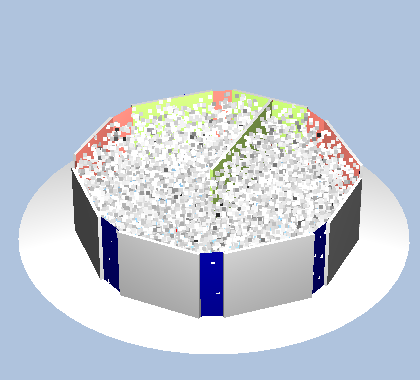
\includegraphics[width=1.5in]{images/intensity_abs}
        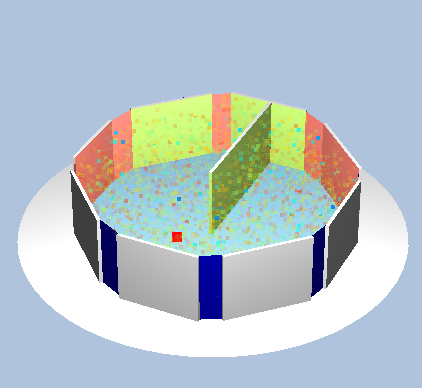
\includegraphics[width=1.5in]{images/hybridVis_abs}
        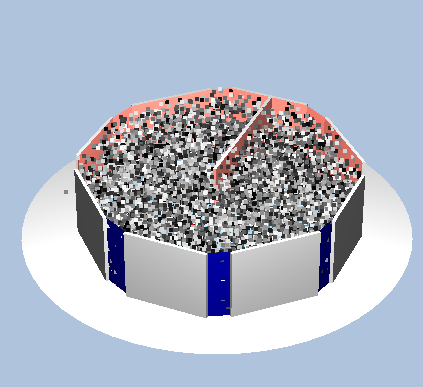
\includegraphics[width=1.5in]{images/freq_noabs}
        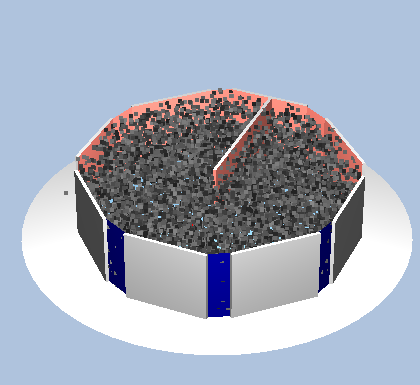
\includegraphics[width=1.5in]{images/intensity_noabs}
        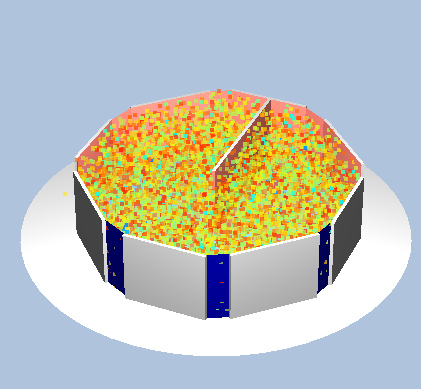
\includegraphics[width=1.5in]{images/hybridVis_noabs}
        \caption{On the top are the results of a room with absorbers installed, and on the bottom with no absorbers installed.}
\end{figure}
%Picture of With in Freq mode, Intensity Mode, Hybrid Mode
%Picture of without floor in Freq mode, Intensity Mode, Hybrid Mode


\section{ Wavefront}
Given user feedback, users stated that seeing the direction of the wave front through color would provide useful in differentiation when a wave hit a wall and changed direction. The result did make it much easier for me to see wavefront emerge as discrete entities that shared similar color. Below are few screen shots of this visualization mode.

	%picture of wave front visualization put 2


%%%%%%%%%%%%%%%%%%%%%%%%%%%%%%%%%%%%%%%%%%%%%%%%%%%%%%%%%%%%%%%%%%%%%%%%%%%%%% %% Conclusions
%%%%%%%%%%%%%%%%%%%%%%%%%%%%%%%%%%%%%%%%%%%%%%%%%%%%%%%%%%%%%%%%%%%%%%%%%%%%%%
\chapter{Conclusions}

Overall, aside from the fully implemented wave particles in 3D, I implemented
phonon mapping as a bases for our simulation. While I would have like to spend time on using an accelerated data structure to speed up the visualizations to interactive frame rates for over 100,000 particles, there is enough content to analysis scene and see see how phonons interact and change at different frequencies depending on the wall material.

Future work lies in the completion of the implementing wave particles, creating a Graphical user interface to control the source sound generated and 
navigate temporally through the architecture space.

%%%%%%%%%%%%%%%%%%%%%%%%%%%%%%%%%%%%%%%%%%%%%%%%%%%%%%%%%%%%%%%%%%%%%%%%%%%%%% %% References
%%%%%%%%%%%%%%%%%%%%%%%%%%%%%%%%%%%%%%%%%%%%%%%%%%%%%%%%%%%%%%%%%%%%%%%%%%%%%%
% The following produces a numbered bibliography where the numbers
% correspond to the \cite commands in the text.
\specialhead{LITERATURE CITED}
\begin{singlespace}
\bibliography{espinm2_thesis}{}
\bibliographystyle{ieeetr}
\end{singlespace}

\end{document}

